% sage_latex_guidelines.tex V1.01, 11 June 2015


% choose journal options here
\documentclass[Royal,sageh,times]{sagej}

\usepackage{moreverb,url}

\usepackage[colorlinks,bookmarksopen,bookmarksnumbered,citecolor=red,urlcolor=red]{hyperref}

\newcommand\BibTeX{{\rmfamily B\kern-.05em \textsc{i\kern-.025em b}\kern-.08em
T\kern-.1667em\lower.7ex\hbox{E}\kern-.125emX}}

\def\volumeyear{2016}



%%%%%%%%%%%%%%%%%%%%%%%
%% User-defined commands
%%%%%%%%%%%%%%%%%%%%%%%

% Operators
\DeclareMathOperator{\Cov}{Cov}
\DeclareMathOperator{\Var}{Var}
\DeclareMathOperator{\E}{\mathbb{E}}
\DeclareMathOperator{\Proba}{\mathbb{P}}

\newcommand{\Covb}[2]{\ensuremath{\Cov\!\left[#1,#2\right]}}
\newcommand{\Eb}[1]{\ensuremath{\E\!\left[#1\right]}}
\newcommand{\Pb}[1]{\ensuremath{\Proba\!\left[#1\right]}}
\newcommand{\Varb}[1]{\ensuremath{\Var\!\left[#1\right]}}

% norm
\newcommand{\norm}[1]{\left\lVert #1 \right\rVert}


% argmin
\DeclareMathOperator*{\argmin}{\arg\!\min}





\setcounter{secnumdepth}{3}


%%%%%%%%%%%%%%%%%%%%%%%
\begin{document}

\runninghead{Raimbault J.}

\title{Indirect Evidence of Network Effects in a System of Cities}

\author{Juste Raimbault\affilnum{1}\affilnum{2}}

\affiliation{\affilnum{1}UMR CNRS 8504 G{\'e}ographie-cit{\'e}s, Paris, France\\
\affilnum{2}UMR-T IFSTTAR 9403 LVMT, Champs-sur-Marne, France}

\corrauth{Juste Raimbault, UMR CNRS 8504 G{\'e}ographie-cit{\'e}s
13 rue du Four,
75006 Paris, France.}

\email{juste.raimbault@polytechnique.edu}

\begin{abstract}
We propose a simple model of urban growth for systems of cities, which investigate in particular the role of physical networks on interdependence of growth rates. Under the assumption of stochastic independence, a generalized non-linear formulation of recursive population growth captures spatial interactions between cities. At the second order, feedback of physical network, introduced as an abstraction of transportation network, is introduced as influencing average growth rates. Model exploration and calibration using large-scale computation and specific algorithms, yield typical characteristics of spatial interaction, such as decay distance, and their evolution in time under non-stationarity hypothesis. Furthermore, network effects are revealed by a fit improvement when adding network module.
\end{abstract}

\keywords{Urban Systems, Urban Growth, Spatial Interactions}

\maketitle


%%%%%%%%%%%%%%%%%%%




%%%%%%%%%%%%%%%%%%%%%%%%
\section*{Introduction}

%%%%%%%%%%%%%%%%%%%%%%%%
\subsection*{Modeling Urban Growth}

Understanding processes driving urban growth is more crucial than ever, as urban population recently crossed the symbolic proportion of half world population~\cite{}.% TODO cite ? 
 Future of world economies and sustainability of future societies seem to be deeply interlinked with the dynamics of urban systems.%cite
 A better knowledge of how cities differentiate, interact and grow is thus a relevant topic both theoretically and for application. Many disciplines have studied models of urban growth with different objectives and taking different aspects into account. Economics still have a difficulty to consider spatial interactions in their models~\cite{krugman1998space}, whereas geography fails to embrace a certain level of complexity. The example of this two disciplines shows how it is difficult to make bridges, as it needed exceptional minds to translate from one to the other (as P. Hall did for Von Thunen work~\cite{taylor2016polymath}) % note : also quote here economic geo/geo economic ?

% broad review from different disciplines point of view
% NOTE : justify scale here (eg not urban sprawl models)

% \cite{rozenfeld2008laws} : systematic empirical study of Urban Growth / Verification of Gibrat's law.



%%%%%%%%%%%%%%%%%%%%%%%%
\subsection*{Urban Growth and Spatial Interaction}

% more refined literature on models of urban growth including space

Some approach of Urban Growth insist on the role of space and spatial interactions. \cite{bretagnolle2000long} already proposed a spatial extension of the Gibrat model. The gravity-based interaction model that~\cite{sanders1992systeme} use to apply concept of Synergetics to cities (getting indeed out of the scope of synergetics by taking expectancies and getting rid of master equation and the probabilistic formulation of trajectories) is also close to this idea of interdependent urban growth, contained physically in the phenomenon of migration between cities. A more refined extension with economic cycles and innovation waves was developed by~\cite{favaro2011gibrat}, yielding a system dynamics version of the core of Simpop models~\cite{pumain2012multi}, which are an other approach to the role of spatial interaction in the growth of urban system

% marius as an extension of Gibrat ? in the deterministic case.


%%%%%%%%%%%%%%%%%%%%%%%%
\subsection*{Urban Growth and Networks}

% idem with networks / transportation networks





% what we propose to do here

We work on simple territorial systems that are country-wide city systems, and more particularly French cities, on a time scale corresponding to that spatial scale, i.e. two last centuries. Taking into account physical networks can improve the understanding of city growth within that system in two ways : a qualitative one, for which the extended model would exhibit qualitative features corresponding to stylized facts empirically observed but that more basic models do not manage to reproduce, and a quantitative way, in the sense that model extension improves explained variance further than the mechanic improvement due to the introduction of supplementary degrees of freedom. If at least one of these is unveiled in our particular case, the evidence will support the theory at these scale and in this context.



The rest of this paper is organized as follows : our model is introduced and formally described in next section ; we then describe results obtained through exploration and calibration of our model on data for french cities, in particular the unveiling of network effects significantly influencing growth processes. We finally discuss interpretations of these results and implications for planning.





%%%%%%%%%%%%%%%%%%%%%%%%%
\section*{Model Description}




\subsection*{From Gibrat to Marius : the dilemma of formulation}

% stochastic vs deterministic formulation ? precise possible formulations and what choice means.

%  - Gabaix \cite{gabaix1999zipf} details stationary distribution of Gibrat model - link with Zipf law. why we do not accept this "explanation" : NOT stationary. depends on time scales to reach stationarity ?
%  - bayesian iterative formulation ? (mcmc)
%  - how does formulation influence ? equivalence in certain cases between stoch-cov and interdependent expectancies ?

Some confusion may arise when surveying at stochastic and deterministic models of urban growth. To what extent is a proposed model ``complex'' and is the simulation of stochasticity necessary ? Concerning Gibrat model and most of its extensions, independence assumptions produce a totally predictable behavior and thus not complex in the sense of exhibiting emergence\footnote{taking e.g. weak emergence, i.e. computational emergence introduced by Bedau~\cite{}}. In particular, the full distribution of random growth models can be analytically at any time~\cite{}, and in the case of studying only first moment, a simple recurrence relation avoids to proceed to any Monte-Carlo simulation. Under these assumptions, it is natural to work with a deterministic model, as it is done by Cottineau with the Marius model~\cite{}.





%%%%%%%%%%%%%%%%%%%%%%
\subsection*{Model description}

We choose to work on a deterministic extension of the Gibrat model, what is equivalent to consider only expectancies in time as explained in the previous subsection. Let $\vec{P}(t)=(P_i(t))_i$ be the population of cities in time. Under Gibrat independence assumptions, we have

\[
\Covb{P_i(t)}{P_j(t)}=0
\]

A linear extended version would write $\vec{P}(t+1)=\mathbf{R}\cdot \vec{P}(t)$ where $\mathbf{R}$ is an independent random matrix of growth rates (identity in the initial case). It yields directly thanks to the independence assumptions that $\Eb{\vec{P}(t+1)}=\Eb{\mathbf{R}}\cdot\Eb{\vec{P}}(t)$. We generalize this linear relation to a non-linear relation that allows to be more consistent regarding some thematic considerations, by taking with denoting $\vec{\mu}(t)=\Eb{\vec{P}(t)}$, the relation $\vec{\mu}(t+1)=f(\vec{\mu}(t))$ (note that in that case, stochastic and deterministic versions are not equivalent anymore\footnote{precisely because of the non-linearity % develop sketch of computation ? - Q under which conditions we can impose a covariance structure that produces interdependencies between expectancies ? seems to be a very broader question, need to do some thinking on that.
}). 
In our case, we take

\begin{equation}
f(\vec{\mu}) = r_0\cdot \mathbf{Id}\cdot \vec{\mu} + \mathbf{G}\left(\vec{\mu}\right)\cdot \mathbf{1} + \mathbf{N}\left(\vec{\mu}\right)
\end{equation}

% TODO recheck formulation and include \Delta t

with $G_{ij} = w_G\cdot \frac{V_{ij}}{<V_{ij}>}$ such that interaction potential follow a gravity-type function given by 

\begin{equation}
V_{ij} = \left(\frac{\mu_i\mu_j}{\sum{\mu_k}^2}\right)^{\gamma_G}\cdot \exp{(-d_{ij}/d_G)}
\end{equation}

and the network effect term is given by


\begin{equation}
N_{i} = w_N \cdot \sum_{kl} \left(\frac{\mu_k\mu_l}{\sum\mu}\right)^{\gamma_N}\exp{(-d_{kl,i})/d_N}
\end{equation}

where $d_{kl,i}$ is distance to shortest path between $k,l$ computed with slope impedance ($Z=\left(1+\alpha/\alpha_0\right)^{n_0}$ with $\alpha_0\simeq 3$). The first component is the pure Gibrat model, that we obtain by setting the weights $w_G = w_N = 0$. The second component captures direct interdependencies between cities, under the form of a separable gravity potential such as the one used in~\cite{sanders1992systeme}. The rationale for the third term, aimed at capturing network effects by expressing a feedback of network flow between cities $k,l$ on the city $i$. Intuitively, a demographic and economic flow physically transiting through a city or in its surroundings is expected to influence its development (through intermediate stops e.g.), this effect being of course dependent on the transportation mode since a high speed line with few stops will induce a \emph{tunnel effect}~\cite{}.% TODO citation tunnel effect.
 Under assumption of non-stationarity, temporal evolution of fitted parameters corresponding to this feedback should therefore contain information on the evolution of transportation modes.


% TODO idea : fixed gravity weight to find significant gravity param -- investigate why saturation at \infty


\paragraph{Model Parameter Space}






%%%%%%%%%%%%%%%%%%%%%%%%
\subsection*{Data}

\paragraph{Population data}

We work with the Pumain-INED historical database for French Cities, which give populations of \emph{Aires Urbaines} (INSEE definition) at time intervals of mostly 5 years, from 1830 to 1995. % TODO precise dates as footnote ?
The latest version of the database, described in~\cite{pumain1986fichier} integrates the definition of Urban Areas, allowing to follow them on long time-period, according to Bretagnole's long time cities ontology~\cite{bretagnolle:tel-00459720} (that constructs a definition of cities as evolving entities which boundaries are not fixed in time).


\paragraph{Stylized facts}

Basic stylized facts can be extracted from such a database, as it has already been widely explored in the literature~\cite{}. %TODO
 We show in figure~\ref{fig:ts-correlations} mean time-series correlation as a function of distance




%%%%%%%%%%%%%%%%%%%%%%%%%
\begin{figure}
\centering
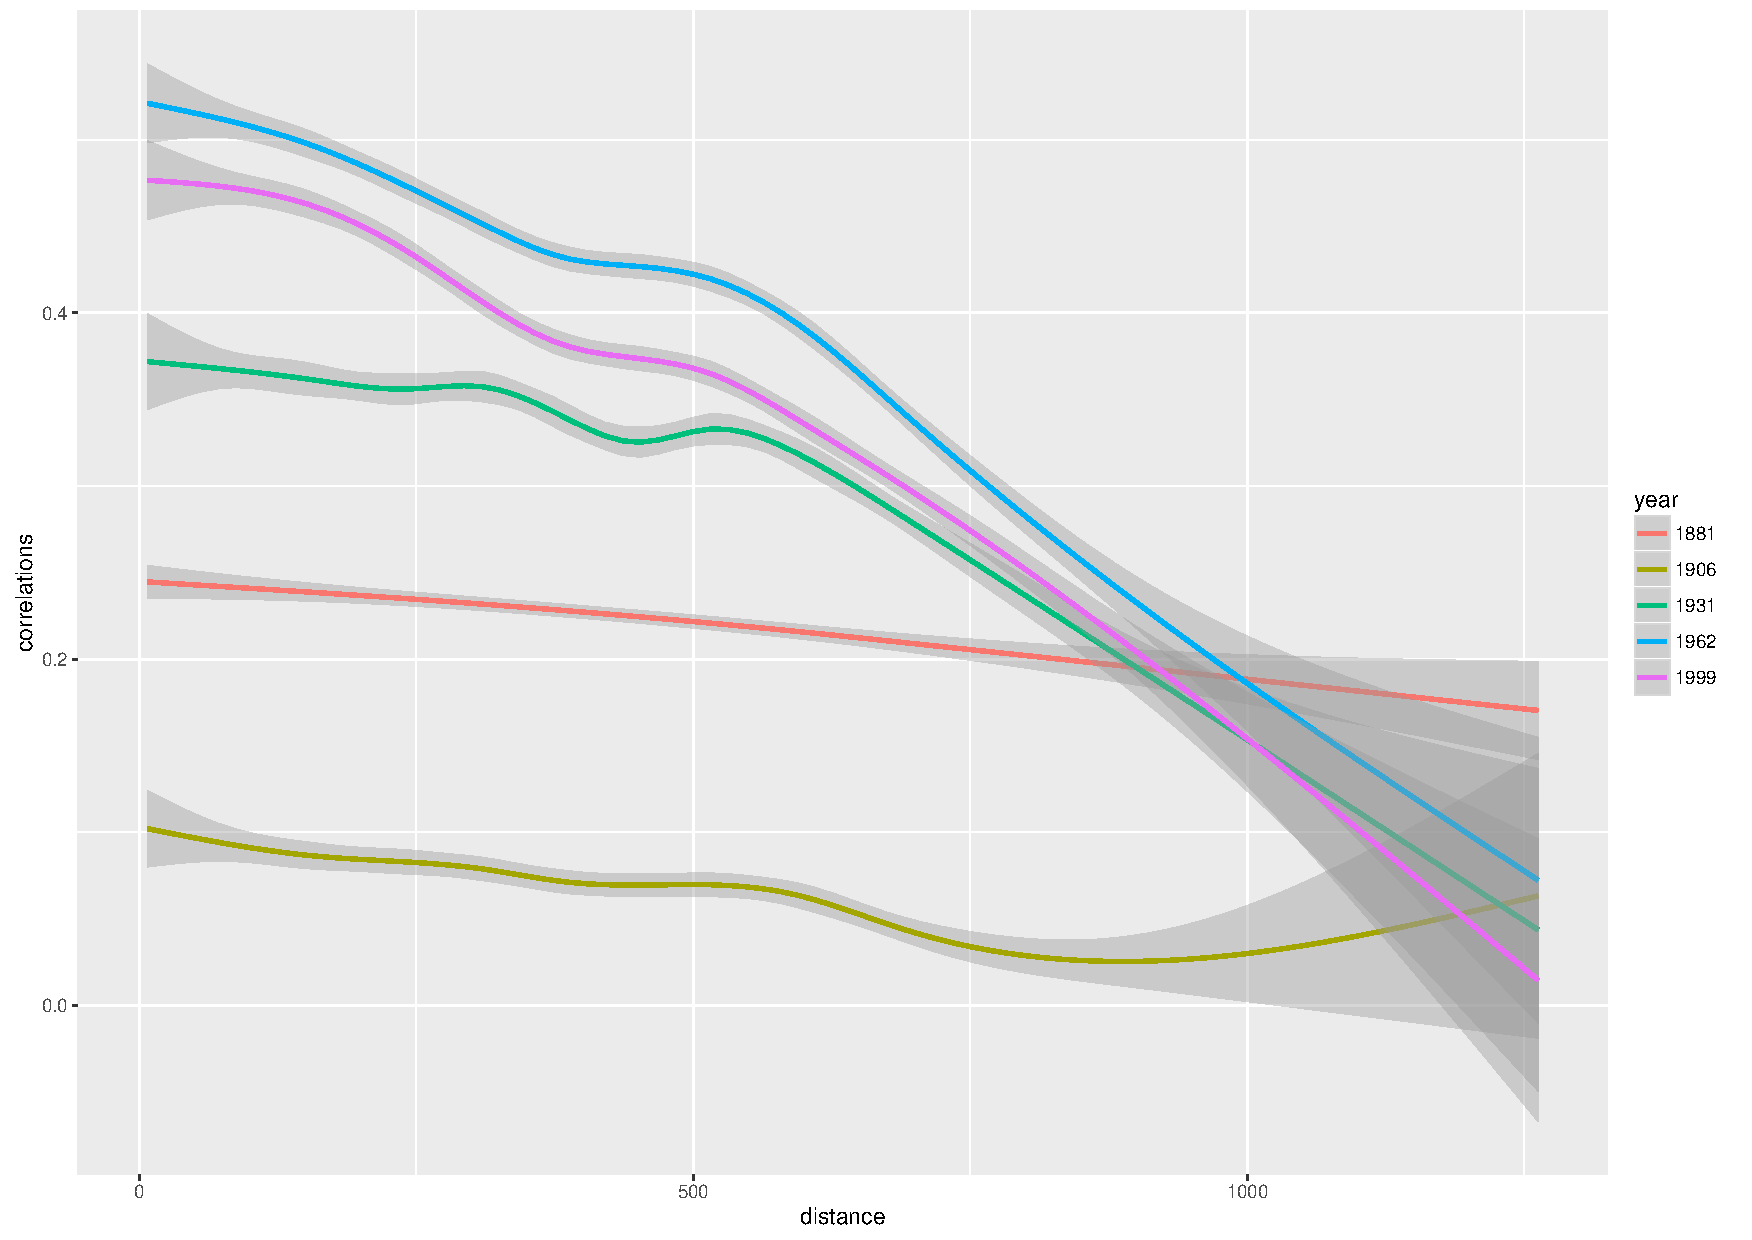
\includegraphics[width=0.8\textwidth]{figures/empirical_tsCorrelations}
\caption{\textbf{Time-series correlations as a function of distance.} Solid line correspond to smoothed correlations, computed between each normalized population time-series, on successive periods. More precisely, we consider overlapping 50 years time-windows finishing respectively in (1881,1906,1931,1962,1999) and compute on each, for each couple of cities $(i,j)$, an estimated correlation $\hat{\rho}_{ij}=\rho\left[\Delta \tilde{P}_i, \Delta \tilde{P}_j\right]$}
\label{fig:ts-correlations}
\end{figure}
%%%%%%%%%%%%%%%%%%%%%%%%%


\paragraph{Physical flows}

As stated above, this modeling exercise focuses on exploring the role of physical flows, whatever the effective shape of the network. We do not need for this reason network data which is furthermore not easily available at different time periods, and physical flows are assumed to take the geographical shortest path that include terrain slope (to avoid geographical absurdities such as cities with a difficult access having an overestimated growth rate). Using the 1km resolution Digital Elevation Model openly available from IGN~\cite{}%cite bdalti
, we construct an impedance field of the form
\[
Z = \left(1 + \frac{\alpha}{\alpha_0}\right)^{n_0}
\]

We took fixed parameter values $\alpha_0 = 3$ (corresponding to approximatively a 5\% slope) and $n_0 = 3$. Supplementary Material S1 justifies this choice by investigating the sensibility of paths to these parameters.

% TODO : supplementary material showing paths for different param values ?



\paragraph{A semi-parametrized model}

Our model is assumed as hybrid as it relies on semi-parametrization on real data. It could be possible to be a full toy-model, initial configuration and physical environment being constructed as synthetic data. As~\cite{raimbault2016generation} points out, it should even be a step in an extensive study of model, using synthetic data to unveil sensibility of dynamics to meta-parameters defining setup. This enterprise is however out of the scope of this paper, as we aim here to extract advanced stylized facts from a dataset, and we focus therefore on the semi-parametrized version of the model.



%%%%%%%%%%%%%%%%%%%%%%%%%
\subsection*{Model Evaluation}
% this subsection AFTER data as it is thanks to data that the model is semi-parametrized

We work on an explanatory rather than an exploratory model, and indicators to evaluate model outputs are therefore not linked to a performance of trajectories or obtained final states, but to a distance to phenomenon we want to explain, i.e. the data. We use therefore the following complementary indicators :

\begin{itemize}
\item Logarithms of mean-square error
\item Mean-square error on logarithms
\end{itemize}







%%%%%%%%%%%%%%%%%%%%%%%%%
\section*{Results}



%%%%%%%%%%%%%%%%%%%%%%%%%%%
\subsection*{Implementation}

Data preprocessing, result processing and models profiling are implemented in R. For performances reasons and an easier integration into the OpenMole software for model exploration described by~\cite{reuillon2013openmole}, a \texttt{scala} version was also developed. The typical question of trade-off between implementation performance and interoperability appeared quickly as an issue, as a blind exploration and calibration can difficultly provide useful thematic conclusions for that kind of model. Finding an improvement in model fit among one parameter dimension is significant if the geographical situation is visualized and the improvement is confirmed as reasonable and not an absurdity.


%%%%%%%%%%%%%%%%%%%
\begin{figure}
\centering
% figures : netlogo interface / typical output ?
\caption{Example of output of the model. The graphical interface allows to explore interactively on which cities changes operate after a parameter change, what is necessary to interpret raw calibration results.}
\end{figure}
%%%%%%%%%%%%%%%%%%%




%%%%%%%%%%%%%%%%%%%%%%%%%%%
\subsection*{Model Exploration}

% qualitative behavior : hierarchy inversions/ trajectories of normalized populations (cf papier Denise Anne etc)
% need of synthetic data ?



%%%%%%%%%%%%%%%%%%%%
\begin{figure}
\centering
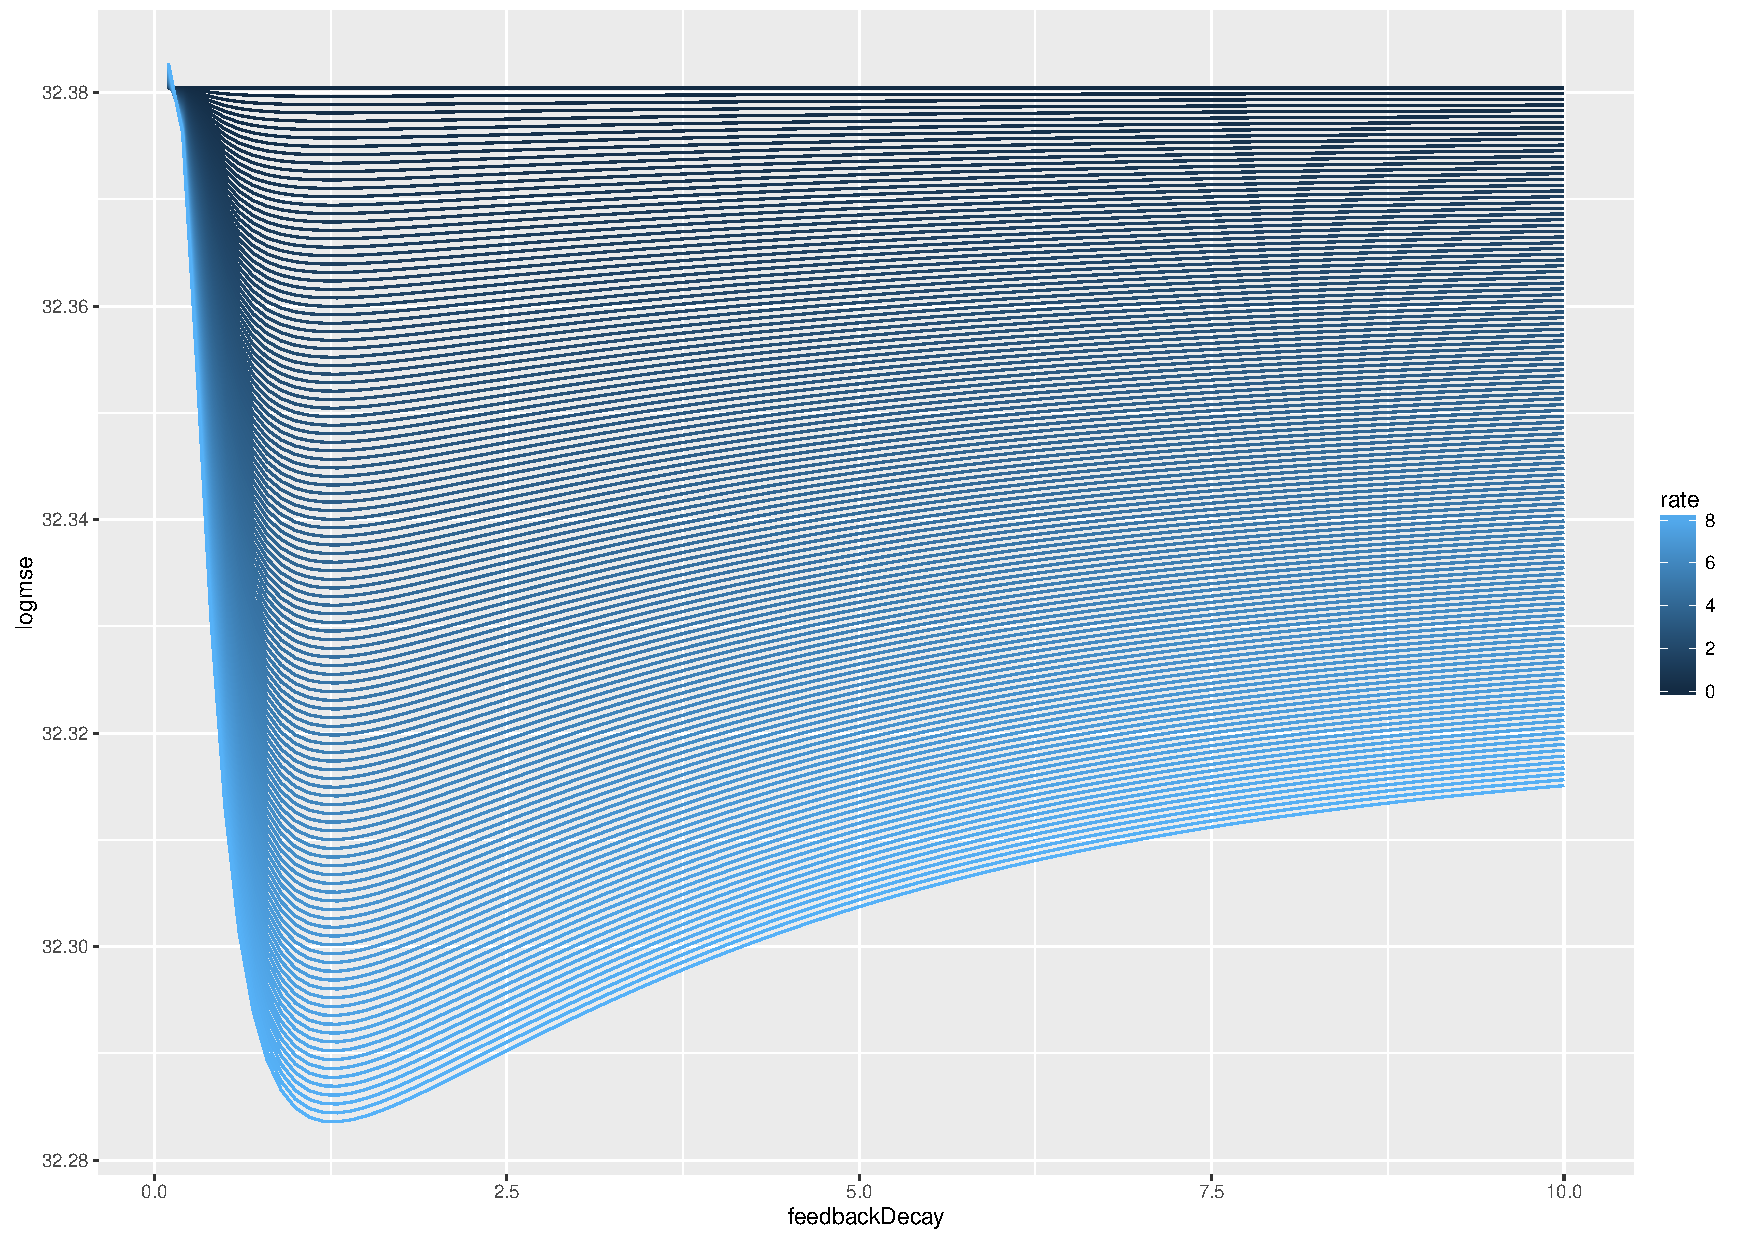
\includegraphics[width=0.48\textwidth]{figures/logmse-feedbackDecay_ZOOM}
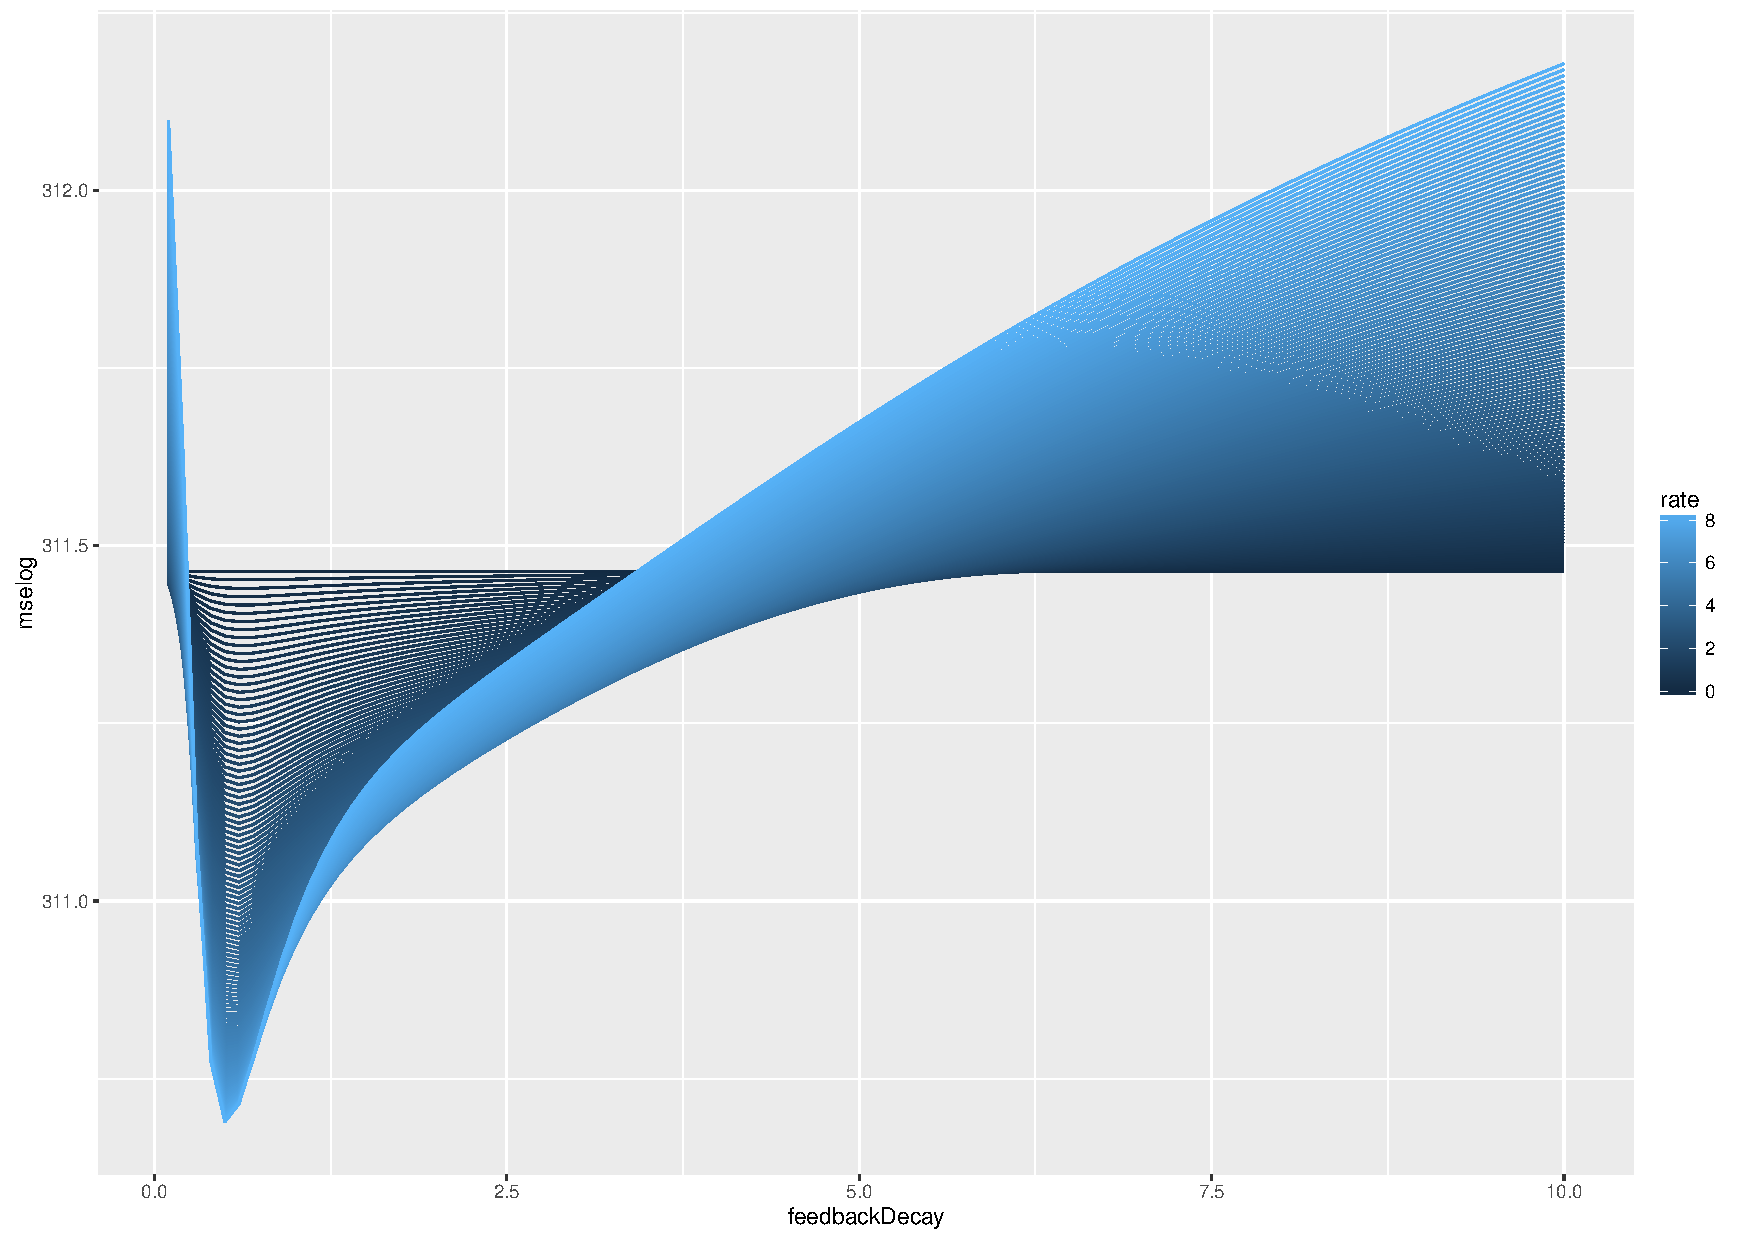
\includegraphics[width=0.48\textwidth]{figures/mselog-feedbackDecay_ZOOM}\\
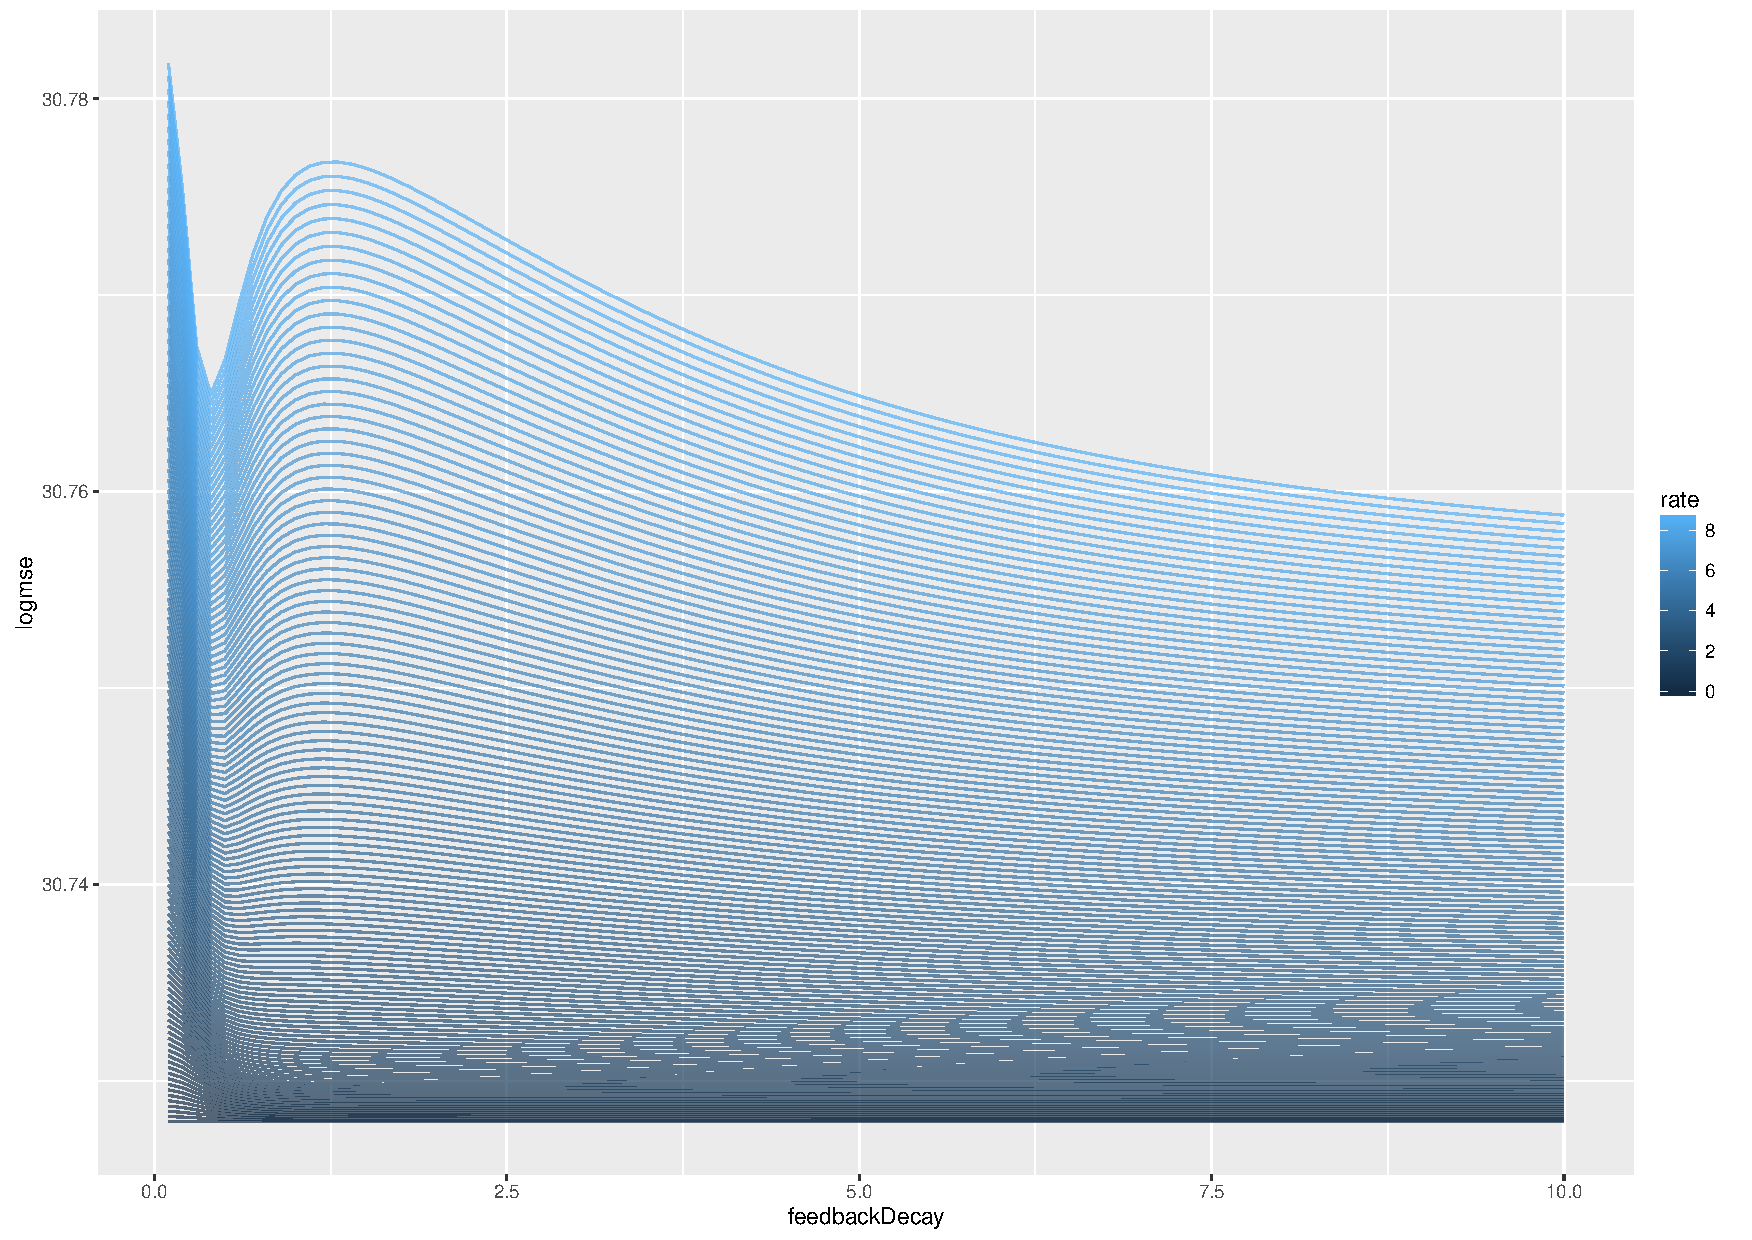
\includegraphics[width=0.48\textwidth]{figures/logmse-feedbackDecay_ZOOM_fixedgravity}
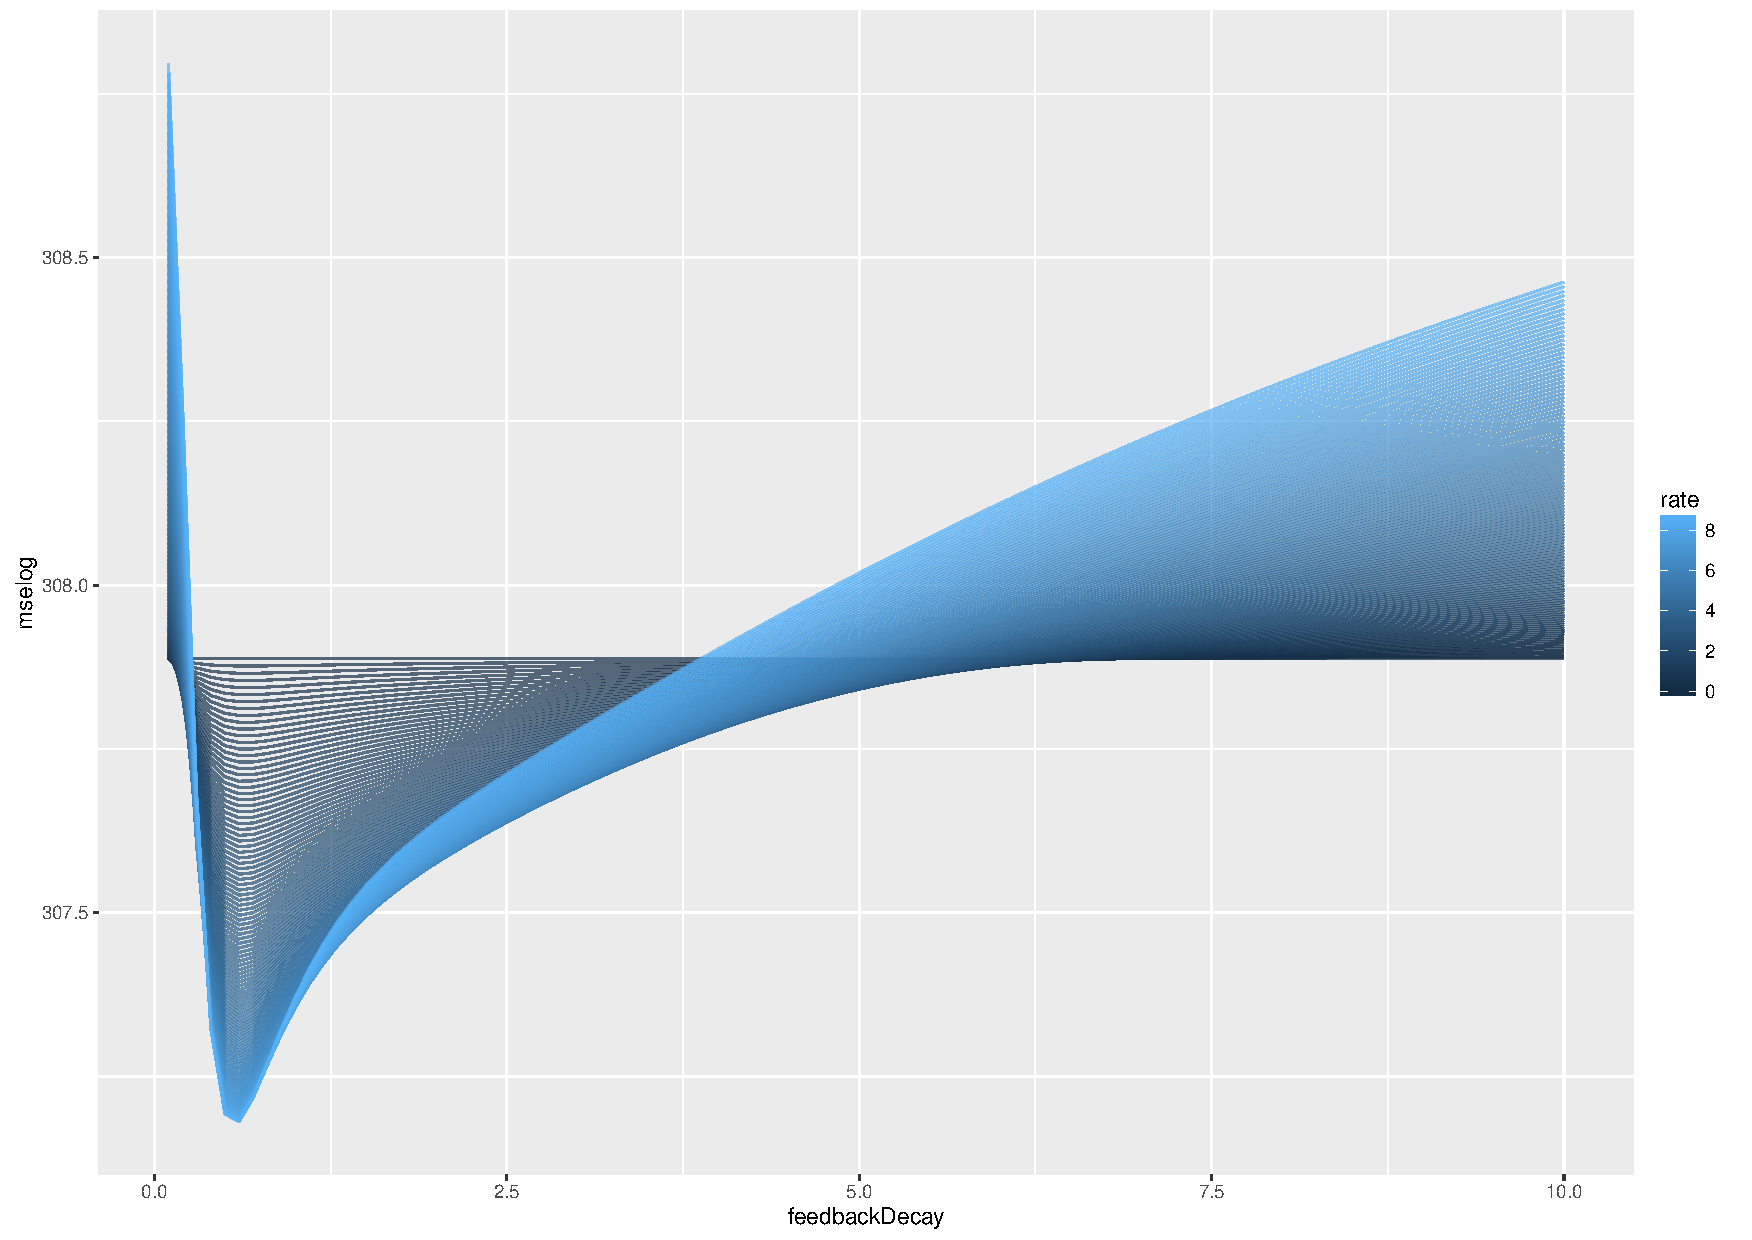
\includegraphics[width=0.48\textwidth]{figures/mselog-feedbackDecay_ZOOM_fixedgravity}
\caption{Evidence of network effects revealed by model exploration. Feedback with fixed gravity : first evidences of network effects ; confirmed with effect of $\alpha_0$}
\end{figure}
%%%%%%%%%%%%%%%%%%%%







%%%%%%%%%%%%%%%%%%%%%%%%%%%
\subsection*{Model Calibration}



\paragraph{Calibration using Genetic Algorithms}


The optimization problem associated to model calibration does not present features allowing an easy solving (closed-form of a likelihood function, convexity or sparsity of the optimization problem, etc.), we must rely on alternative techniques to solve it. Brute force grid search is rapidly limited by the dimensionality curse


%%%%%%%%%%%%%%%%%%%%%%%%%%%
\begin{figure}
\centering
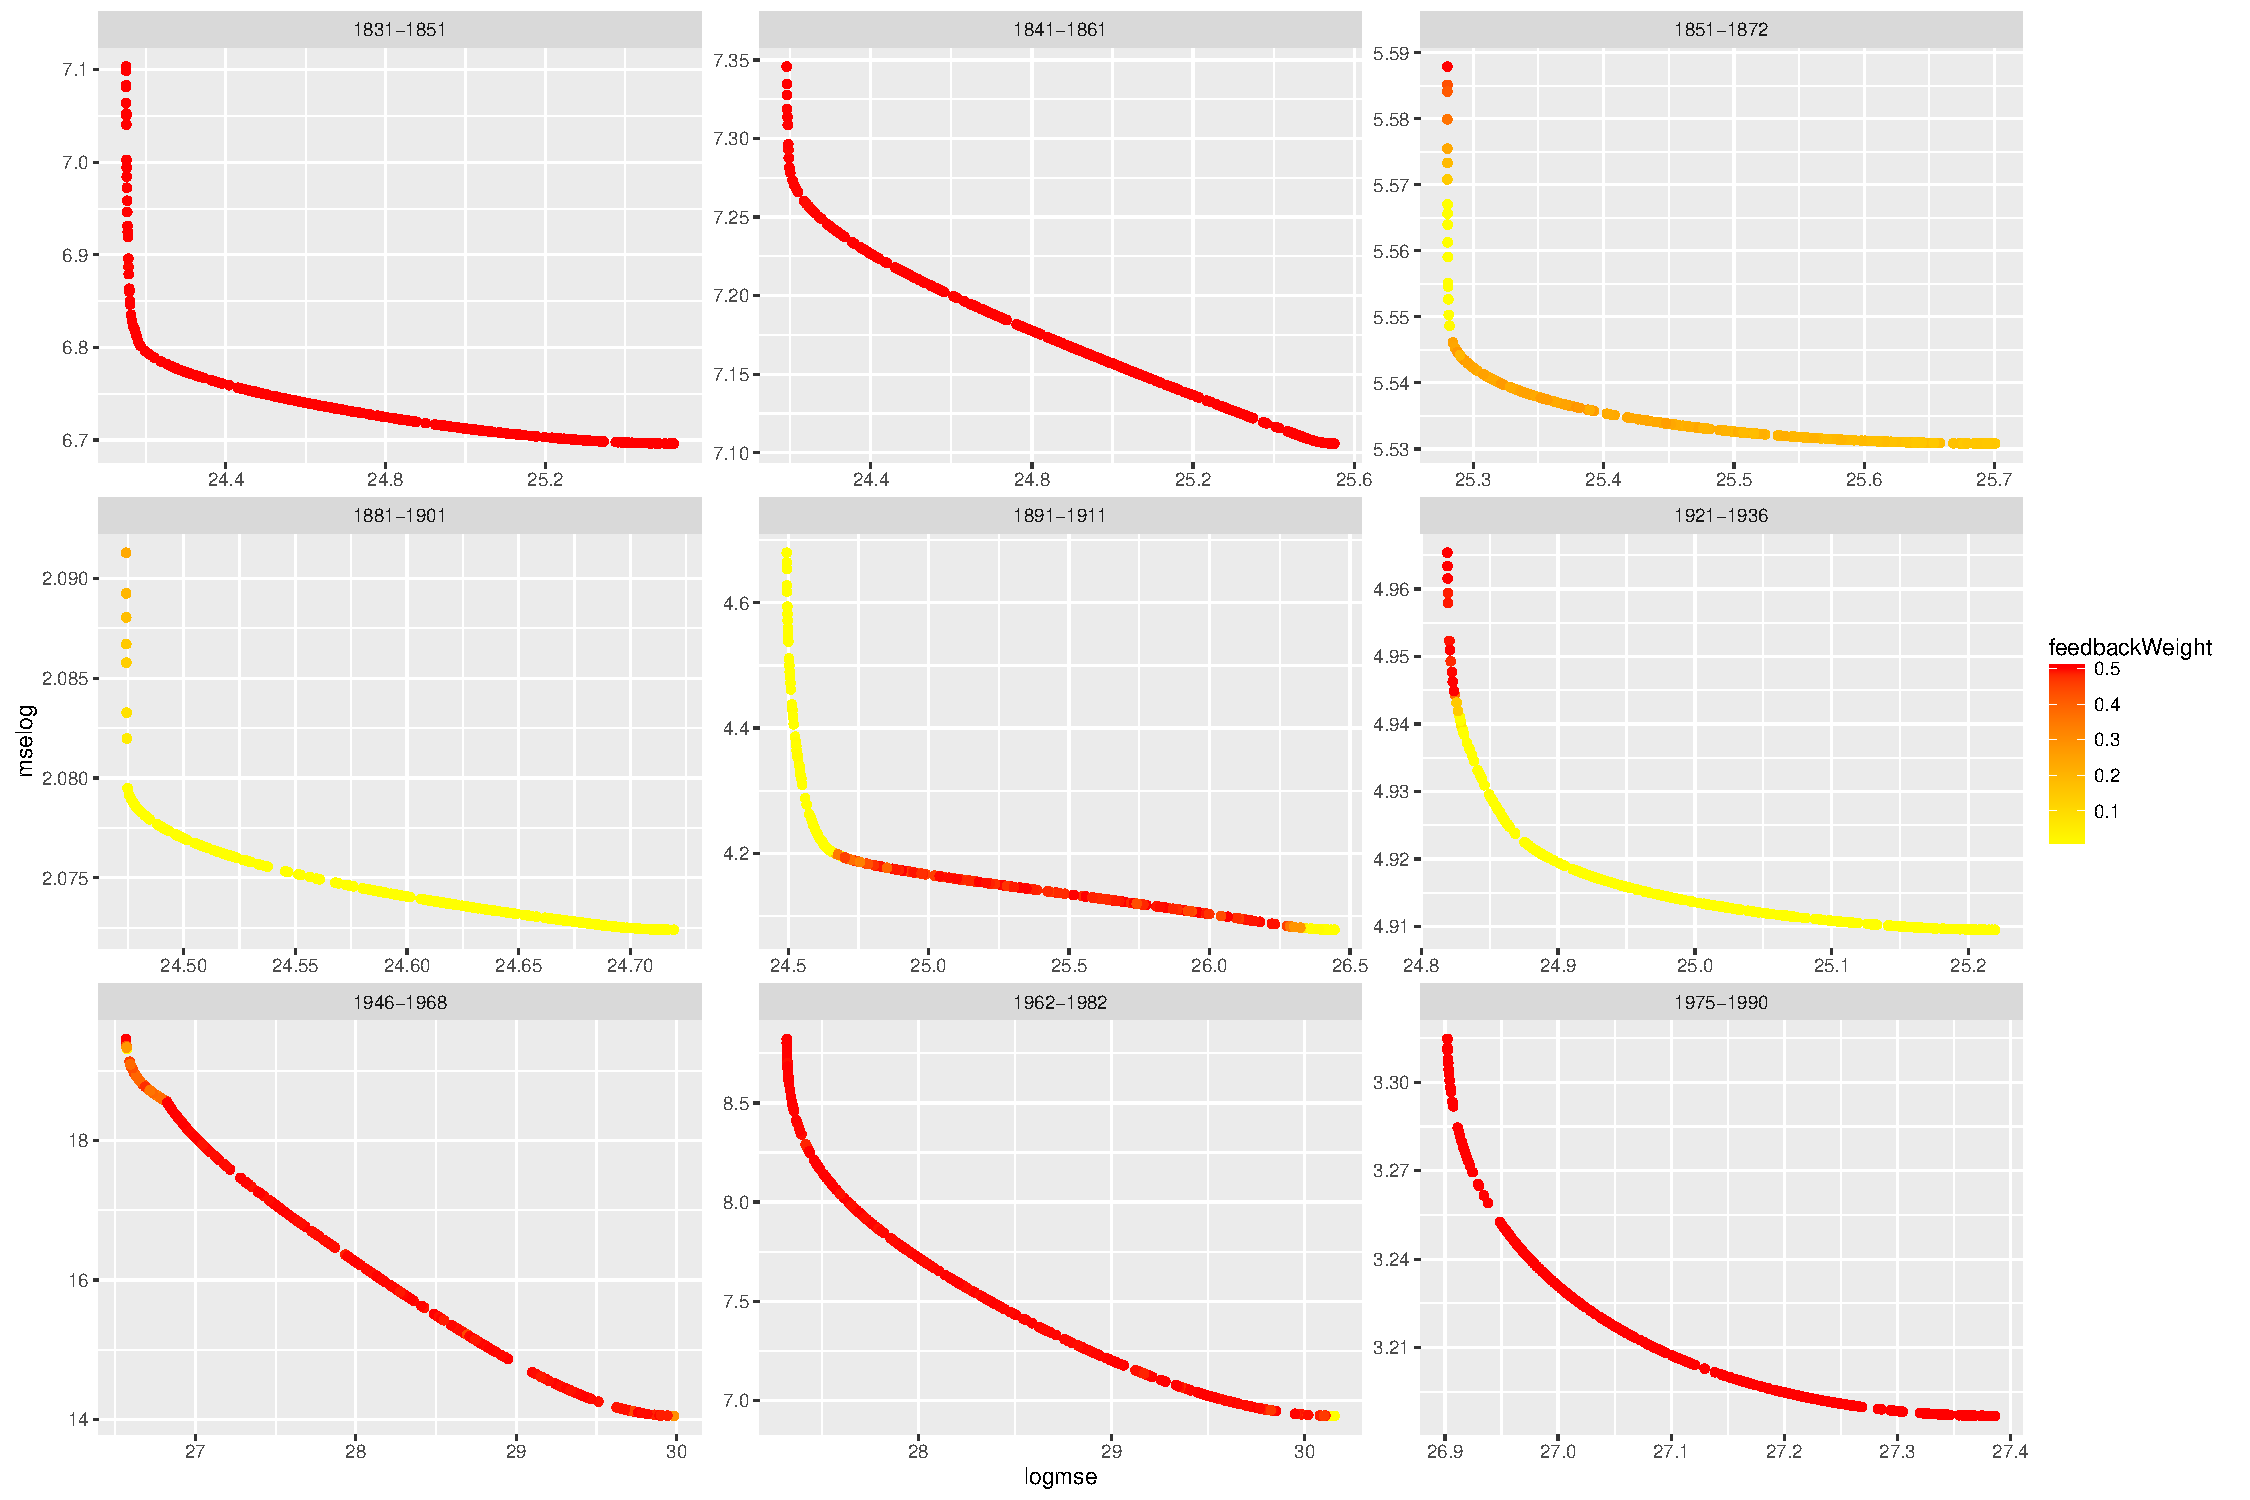
\includegraphics[width=\textwidth]{figures/allperiods_feedbackWeight}
\caption{\textbf{Pareto fronts for bi-objective calibration.} Steady-state populations are obtained using Island Genetic Algorithm embedded in \texttt{OpenMole}, with parameters, and on independent time periods as detailed in text. We show  corresponding parameter values for $w_N$, for the gravity-only model (Top) and the full model (Bottom). Full graphs are available in Supplementary materials.}
\end{figure}
%%%%%%%%%%%%%%%%%%%%%%%%%%%



\paragraph{Quantifying overfitting : Empirical AIC}

% here put empirical AIC ?

% \cite{2017arXiv170108673P} : selecting number of states in HMM, analog ?
% \cite{biernacki2000assessing} : other type of computational aic-type indicator.

A large part of statistical models allow to compute tools for model comparison and selection, in particular to take into account possible overfitting due to additional degrees of freedom. The Akaike Information Criterion provides the gain in information between two models, and many extensions have been proposed since~\cite{}.% TODO cite AIC
Note that cross-validation type of methods are not suitable to our case because of the small size of the dataset. We can formalize the proposed method based on the intuitive idea of approaching models of simulation by statistical models and using the corresponding AIC under certain validity conditions. Let $(X,Y)$ be the data and observations. Computational models are functions $(X,\alpha_k) \mapsto M_{\alpha_k}^{(k)}(X)$ mapping data values to a random variable. What is seen as data and parameters is somehow arbitrary but is separated in the formulation as corresponding dimensions will have different roles. We assume the model has been fitted to data in the sense that an heuristic has been used to approximate $\alpha^{\ast}_k = \argmin_{\alpha_k}\norm{M_{\alpha_k}^{(k)}(X) - Y}$. The gain of information between two computational models is not directly accessible and we propose an indirect way, through the fitting of statistical models. For all computational model, a large set of statistical models with similar degree of freedom are fitted. % TODO not clear here 
Let $S_k$ be the statistical models fitting best $M^{(k)}_{\alpha^{\ast}_k}(X)$. We can compute

\[
\Delta D_{KL} \left(M^{(1)}|M^{(2)}\right) = \Delta D_{KL} \left(S^{(1)}|S^{(2)}\right) + \left[ \Delta D_{KL} \left(S^{(2)}|M^{(1)}\right) + \Delta D_{KL} \left(S^{(1)}|M^{(2)}\right) \right]
\]

Under certain assumptions, the order of magnitude of second term appears to be negligible. More precisely, with $s^{(k)}=M^{(k)}-S^{(k)}$, we have

\[
\norm{\int f \log{\left(\frac{S^{(k)}}{M^{(k')}}\right)}} = \norm{\int f \log{\left(1 + \frac{s^{(k)}}{M^{(k')}}\right)}}
\]


%%%%%%%%%%%%%%%%%%%%%%%%%%%
\section*{Discussion}

%%%%%%%%%%%%%%%%%%%%%%%%%%%
% 
%  - how this example illustrates well the theory
%  - reflexions on iterative calibration, here ?
%  - multimodeling etc
%  - back to the simple arg ? rgs argument also ?
%  - not tested on other system of cities
%  - no network data -> development with train ?
%
%



%%%%%%%%%%%%%%%%%%%%%%%%%%%
\subsection*{Theoretical implications}


We propose to support our hypothesis that \textit{physical transportation networks are necessary to explain the morphogenesis of territorial systems} (aka \textit{Network Necessity}) by showing on a relatively simple case that the integration of physical networks into some models effectively increase their explanative power (being careful on the precise definition of model improvement to avoid overfitting).

% cite theoretical draft here ?

%%



%%%%%%%%%%%%%%%%%%%%%%%%%%%
\subsection*{Methodological implications}





%%%%%%%%%%%%%%%%%%%%%%%%%%%
\subsection*{Further developments}


\paragraph{Specificity of the Urban System}

The model has not yet been tested on other urban systems and other temporalities.



\paragraph{Towards co-evolutive models of cities and transportation networks}

Our focus on network effects remains quite limited since (i) we do not consider an effective infrastructure but abstract flows only, and (ii) we do not take into account the possible network evolution, due to technical progresses (\cite{bretagnolle2000long}) and infrastructure growth in time. An ambitious but necessary development would be the inclusion of both in a model of co-evolution between urban growth and transportation network growth, in order to investigate to what extent the refinement of network spatial structure and network dynamics can improve the explanation of urban system dynamics. It has been shown by \cite{raimbault2016models} that disciplinary compartmentalization may be at the origin of the relative absence of such type of models in the literature.




%%%%%%%%%%%%%%%%%%%%%%%%%%%
\section*{Conclusion}






%%%%%%%%%%%%%
\begin{acks}
The author would like to thank
\end{acks}
%%%%%%%%%%%%%




%%%%%%%%%%%%%
%% Biblio
%%%%%%%%%%%%%
\bibliographystyle{SageH}
\bibliography{biblio}



%%%%%%%%%%%%%
%% Supplementary materials
%%%%%%%%%%%%%



%%%%%%%%%%%%%
\section*{Physical Flows Parametrization}

We show in Fig.~\ref{fig:shortest-path-densities} footprints of shortest paths, revealing how different values make the path more or less realistic regarding the elevation map. A rather rough validation can also been done by comparing these with the actual current shortest paths by the road network. These are computed using the road network dataset provided by~\cite{} % dataverse simplified road network
and which construction is detailed in~\cite{}. % working paper version of datapaper ?
For each path, we can define a measure of geographical distance as, given $(\vec{l}_i (s), \vec{l}_j (s))$ normalized linear parametrization of two paths $(p_i,p_j)$, by

\[
d(p_i,p_j) = \int_{s=0}^1 \norm{\vec{l}_i (s) - \vec{l}_j (s)} ds
\] 

We show in Fig.~\ref{fig:paths-geodistance}


%%%%%%%%%%%%%
\begin{figure}

\caption{Densities of shortest paths, computed with the 1225 shortest between all 50 cities included in the dataset, for different values of parameters $(\alpha_0,n_0)$.}
\label{fig:shortest-path-densities}
\end{figure}
%%%%%%%%%%%%%


%%%%%%%%%%%%%
\begin{figure}

\caption{Errors on shortest paths using the geographical path heuristic. (a) Distribution of integrated distance between paths. (b) Density maps for both heuristic and real paths.}
\label{fig:paths-geodistance}
\end{figure}
%%%%%%%%%%%%%


%%%%%%%%%%%%%
%\section*{Reproducibility}

%%%%%%%%%%
% - DATA available where ?
% - give git commits that have produced exactly the results.
% -> not necessary, and the subrepo should be cloned/anonymized. put that in main text.









\end{document}
























%%%%%%%%%%%%%%%%%%%%
%% Templates
%%%%%%%%%%%%%%%%%%%%




%
%\subsection{Remarks}
%\begin{enumerate}
%\item[(i)] In \verb"\runninghead" use `\textit{et~al.}' if there
%are three or more authors.
%
%\item[(ii)] For multiple author papers please note the use of \verb"\affilnum" to
%link names and affiliations. The corresponding author details need to be included using the
%\verb+\corrauth+ and \verb+\email+ commands.
%
%\item[(iii)] For submitting a double-spaced manuscript, add
%\verb"doublespace" as an option to the documentclass line.
%
%\item[(iv)] The abstract should be capable of standing by itself,
%in the absence of the body of the article and of the bibliography.
%Therefore, it must not contain any reference citations.
%
%\item[(v)] Keywords are separated by commas.
%
%\item[(vi)] If you are submitting to a \textit{SAGE} journal that requires numbered sections (for example, IJRR), please add the command
%  \verb+\setcounter{secnumdepth}{3}+ just above the \verb+\begin{document}+ line.
%
%\end{enumerate}
%
%




%
%
%\section{The article header information}
%The heading for any file using \textsf{\journalclass} is shown in
%Figure~\ref{F1}. You must select options for the trim/text area and
%the reference style of the journal you are submitting to.
%The choice of \verb+options+ are listed in Table~\ref{T1}.
%
%\begin{table}[h]
%\small\sf\centering
%\caption{The choice of options.\label{T1}}
%\begin{tabular}{lll}
%\toprule
%Option&Trim&Columns\\
%\midrule
%\texttt{shortAfour}& 210 $\times$ 280 mm& Double column\\
%\texttt{Afour} &210 $\times$ 297 mm& Double column\\
%\texttt{MCfour} &189 $\times$ 246 mm& Double column\\
%\texttt{PCfour} &170 $\times$ 242 mm& Double column\\
%\texttt{Royal} &156 $\times$ 234 mm& Single column\\
%\texttt{Crown} &7.25 $\times$ 9.5 in&Single column\\
%\bottomrule
%\end{tabular}\\[10pt]
%\begin{tabular}{ll}
%\toprule
%Option&Reference style\\
%\midrule
%\texttt{sageh}&SAGE Harvard style (author-year)\\
%\texttt{sagev}&SAGE Vancouver style (superscript numbers)\\
%\texttt{sageapa}&APA style (author-year)\\
%\bottomrule
%\end{tabular}
%\end{table}
%
%For example, if your journal is short A4 sized, uses Times fonts and has Harvard style references then you would need\\
%{\small\verb+\documentclass[ShortAfour,times,sageh]{sagej}+}
%
%Most \textit{SAGE} journals are published using Times fonts but if for any reason you have a problem using Times you can
%easily resort to Computer Modern fonts by removing the
%\verb"times" option.





%\begin{figure*}
%\setlength{\fboxsep}{0pt}%
%\setlength{\fboxrule}{0pt}%
%\begin{center}
%\begin{boxedverbatim}
%\documentclass[<options>]{sagej}
%
%\begin{document}
%
%\runninghead{<Author surnames>}
%
%\title{<Initial capital only>}
%
%\author{<An Author\affilnum{1},
%Someone Else\affilnum{2} and
%Perhaps Another\affilnum{1}>}
%
%\affiliation{<\affilnum{1}First and third authors' affiliation\\
%\affilnum{2}Second author affiliation>}
%
%\corrauth{<Corresponding author's name and full postal address>}
%
%\email{<Corresponding author's email address>}
%
%\begin{abstract}
%<Text>
%\end{abstract}
%
%\keywords{<List keywords>}
%
%\maketitle
%
%\section{Introduction}
%.
%.
%.
%\end{boxedverbatim}
%\end{center}
%\caption{Example header text.\label{F1}}
%\end{figure*}



%
%
%
%
%
%%%%%%%%%%%%%%%%%%%%%%%%
%\section{The body of the article}
%
%\subsection{Mathematics} \textsf{\journalclass} makes the full
%functionality of \AmS\/\TeX\ available. We encourage the use of
%the \verb"align", \verb"gather" and \verb"multline" environments
%for displayed mathematics. \textsf{amsthm} is used for setting
%theorem-like and proof environments. The usual \verb"\newtheorem"
%command needs to be used to set up the environments for your
%particular document.
%
%\subsection{Figures and tables} \textsf{\journalclass} includes the
%\textsf{graphicx} package for handling figures.
%
%Figures are called in as follows:
%\begin{verbatim}
%\begin{figure}
%\centering
%\includegraphics{<figure name>}
%\caption{<Figure caption>}
%\end{figure}
%\end{verbatim}
%
%For further details on how to size figures, etc., with the
%\textsf{graphicx} package see, for example, \cite{R1}
%or \cite{R3}.
%
%The standard coding for a table is shown in Figure~\ref{F2}.
%
%\begin{figure}
%\setlength{\fboxsep}{0pt}%
%\setlength{\fboxrule}{0pt}%
%\begin{center}
%\begin{boxedverbatim}
%\begin{table}
%\small\sf\centering
%\caption{<Table caption.>}
%\begin{tabular}{<table alignment>}
%\toprule
%<column headings>\\
%\midrule
%<table entries
%(separated by & as usual)>\\
%<table entries>\\
%.
%.
%.\\
%\bottomrule
%\end{tabular}
%\end{table}
%\end{boxedverbatim}
%\end{center}
%\caption{Example table layout.\label{F2}}
%\end{figure}
%
%\subsection{Cross-referencing}
%The use of the \LaTeX\ cross-reference system
%for figures, tables, equations, etc., is encouraged
%(using \verb"\ref{<name>}" and \verb"\label{<name>}").
%
%\subsection{End of paper special sections}
%Depending on the requirements of the journal that you are submitting to,
%there are macros defined to typeset various special sections. \pagebreak
%
%The commands available are:
%\begin{verbatim}
%\begin{acks}
%To typeset an
%  "Acknowledgements" section.
%\end{acks}
%\end{verbatim}
%\begin{verbatim}
%\begin{biog}
%To typeset an
%  "Author biography" section.
%\end{biog}
%\end{verbatim}
%\begin{verbatim}
%\begin{biogs}
%To typeset an
%  "Author Biographies" section.
%\end{biogs}
%\end{verbatim}
%\begin{verbatim}
%\begin{dci}
%To typeset a "Declaration of
%  conflicting interests" section.
%\end{dci}
%\end{verbatim}
%\begin{verbatim}
%\begin{funding}
%To typeset a "Funding" section.
%\end{funding}
%\end{verbatim}
%\begin{verbatim}
%\begin{sm}
%To typeset a
%  "Supplemental material" section.
%\end{sm}
%\end{verbatim}
%
%\subsection{Endnotes}
%Most \textit{SAGE} journals use endnotes rather than footnotes, so any notes should be coded as \verb+\endnote{<Text>}+.
%Place the command \verb+\theendnotes+ just above the Reference section to typeset the endnotes.
%
%To avoid any confusion for papers that use Vancouver style references,  footnotes/endnotes should be edited into the text.
%


%
%\subsection{References}
%Please note that the files \textsf{SageH.bst} and \textsf{SageV.bst} are included with the class file
%for those authors using \BibTeX. For APA style references please use \textsf{mslapa.bst} which should be part of most modern \TeX\ distributions.
%
%See the above instructions regarding choosing the correct reference option.
%
%%\section{Support for \textsf{\journalclass}}
%%We offer on-line support to participating authors. Please contact
%%us via e-mail at \dots
%%
%%We would welcome any feedback, positive or otherwise, on your
%%experiences of using \textsf{\journalclass}.
%




%
%\section{Copyright statement}
%Please  be  aware that the use of  this \LaTeXe\ class file is
%governed by the following conditions.
%
%\subsection{Copyright}
%Copyright \copyright\ \volumeyear\ SAGE Publications Ltd,
%1 Oliver's Yard, 55 City Road, London, EC1Y~1SP, UK. All
%rights reserved.
%
%\subsection{Rules of use}
%This class file is made available for use by authors who wish to
%prepare an article for publication in a \textit{SAGE Publications} journal.
%The user may not exploit any
%part of the class file commercially.
%
%This class file is provided on an \textit{as is}  basis, without
%warranties of any kind, either express or implied, including but
%not limited to warranties of title, or implied  warranties of
%merchantablility or fitness for a particular purpose. There will
%be no duty on the author[s] of the software or SAGE Publications Ltd
%to correct any errors or defects in the software. Any
%statutory  rights you may have remain unaffected by your
%acceptance of these rules of use.
%
%



%
%
%\begin{thebibliography}{99}
%\bibitem[Kopka and Daly(2003)]{R1}
%Kopka~H and Daly~PW (2003) \textit{A Guide to \LaTeX}, 4th~edn.
%Addison-Wesley.
%
%\bibitem[Lamport(1994)]{R2}
%Lamport~L (1994) \textit{\LaTeX: a Document Preparation System},
%2nd~edn. Addison-Wesley.
%
%\bibitem[Mittelbach and Goossens(2004)]{R3}
%Mittelbach~F and Goossens~M (2004) \textit{The \LaTeX\ Companion},
%2nd~edn. Addison-Wesley.
%
%\end{thebibliography}
%
%





